\documentclass{uninove-ppgi} %courier ou times

\begin{document}
\lstset{
    language=xml,
    tabsize=3,
    frame=shadowbox,
    rulesepcolor=\color{gray},
    xleftmargin=20pt,
    framexleftmargin=15pt,
    keywordstyle=\color{blue}\bf,
    commentstyle=\color{OliveGreen},
    stringstyle=\color{red},
    numbers=left,
    numberstyle=\tiny,
    numbersep=5pt,
    breaklines=true,
    showstringspaces=false,
    basicstyle=\footnotesize,
    emph={food,name,price},emphstyle={\color{magenta}}
}

% parametros de capa e folha de rosto (é necessário configurar todos)
\Universidade{UNIVERSIDADE NOVE DE JULHO - UNINOVE}
\Programa{PROGRAMA DE PÓS GRADUAÇÃO EM INFORMÁTICA E GESTÃO DO CONHECIMENTO - PPGIGC}
\Autor{NOME DO DISCENTE}

\Titulo{TÍTULO DO TRABALHO}
\Tipoexame{qualificação} % qualificação ou defesa
\Titulacao{Doutor} % Mestre ou Doutor
\Orientador{Dr(a). Nome do(a) Orientador(a)}
\Coorientador{Dr(a). Nome do(a) Coorientador(a)} % Se não houver, deve ser comentada a linha no arquivos uninove-ppgi.cls

% Descomentar as linhas abaixo e no arquivo "uninove-ppgi.cls" para utilizar na disciplina de seminários
%\Ingresso{XX/20XX}
%\Linha{LP1 - Modelagem e Otimização Computacional}
%\Linha{LP2 - Sistemas Inteligentes}
%\Linha{LP3 - Gestão da Tecnologia da Informação e Conhecimento}
\Ano{202X} % inserir o ano correspondente

% gera a capa
\capa

% gera folha de rosto
\folharosto

% Ficha catalográfica
%\includepdf[pages=-]{fichaCatalografica.pdf}

% Ficha de aprovação
% \includepdf[pages=-]{parecer_assinado.pdf}

% ##################### Início dos elementos pré-textuais ############################

% Dedicatória (Opcional)
\centeredchapterstyle
% !TEX root = ..\main.tex

\begin{dedicatoria}\vspace*{\fill}
	\begin{flushright}\textbf{\vspace*{\stretch{3}}\\}
		\begin{changemargin}{+5cm}{0cm}
			Tempor amet voluptate laborum aute cillum laborum velit enim commodo consequat est. Eiusmod consectetur proident ad dolor laboris consequat sunt est veniam proident. Aute eu elit fugiat eiusmod id enim dolor. Esse officia id proident anim. Id quis laboris quis pariatur proident.
		\end{changemargin}
	\end{flushright}
\end{dedicatoria}

\thispagestyle{empty}
\clearpage

% Agradecimentos (Opcional)
%\chapter*{Agradecimentos}
\centeredchapterstyle
\begin{agradecimentos}
    \noindent Agradecimentos pessoais. \newline

    \noindent Agradecimento ao orientador(a).\newline
    
    \noindent Agradecimento ao coorientador(a).\newline
    
    \noindent Outros agradecimentos.\newline
    
    \noindent À Universidade Nove de Julho (UNINOVE), pela oportunidade da concessão da bolsa de estudos.\newline
    
    \noindent Por fim, outros agradecimentos que não excedam a uma página no total.
\end{agradecimentos}

\thispagestyle{empty}
\clearpage

% Epígrafe (Opcional)
% !TEX root = ..\main.tex

\begin{epigrafe}\vspace*{\fill}
    \begin{center}
    	\begin{flushright}\vspace*{1cm}
            \begin{minipage}{.8\textwidth}
            \begin{flushright}
            		\textit{``Nisi labore ea pariatur quis nulla consectetur ad excepteur ullamco sit. Ea anim nisi amet incididunt deserunt.''}.\\
        		\end{flushright}
        		\begin{flushright}
        		Lorem Ipsum (2001)\\
        		\textit{Poeta}.
        		\end{flushright}
            \end{minipage}
        \end{flushright}
    \end{center}
\end{epigrafe}

% Resumo (Obrigatório)
% !TEX root = ..\main.tex

\PalavrasChave{Palavra 1, Palavra 2, Palavra 3, Palavra 4, Palavra 5, Palavra 6.}
\centeredchapterstyle
\begin{resumo}
    \noindent\textbf{Contexto}: Nisi mollit anim consequat deserunt tempor laboris fugiat sit do. Pariatur duis est incididunt deserunt pariatur quis sint. Consectetur aliqua reprehenderit laborum aute id dolor fugiat. In consequat pariatur officia dolor esse pariatur sit reprehenderit. Duis nostrud proident occaecat non adipisicing officia sit sunt aute. Nulla eiusmod labore elit velit. Labore fugiat dolor sint irure Lorem irure est voluptate dolor magna commodo. \textbf{Objetivo}: Consequat velit incididunt laborum sit reprehenderit ea ex cillum ut ut incididunt veniam veniam id. \textbf{Método}: Deserunt labore labore reprehenderit fugiat dolor Lorem enim consequat ea. Reprehenderit officia id eiusmod voluptate dolor excepteur. Ut adipisicing occaecat laboris minim laborum dolore tempor. Veniam aliqua ad exercitation aute Lorem veniam laborum voluptate anim sunt enim. \textbf{Resultados}: Deserunt labore labore reprehenderit fugiat dolor Lorem enim consequat ea. Reprehenderit officia id eiusmod voluptate dolor excepteur. Ut adipisicing occaecat laboris minim laborum dolore tempor. Veniam aliqua ad exercitation aute Lorem veniam laborum voluptate anim sunt enim. \textbf{Conclusão}: Deserunt labore labore reprehenderit fugiat dolor Lorem enim consequat ea. Reprehenderit officia id eiusmod voluptate dolor excepteur. Ut adipisicing occaecat laboris minim laborum dolore tempor. Veniam aliqua ad exercitation aute Lorem veniam laborum voluptate anim sunt enim.
\end{resumo}

% Abstract (Obrigatório)
% !TEX root = ..\main.tex

\KeyWords{Keyword 1, Keyword 2, Keyword 3, Keyword 4, Keyword 5, Keyword 6.}
\centeredchapterstyle
\begin{abstract}
    \noindent\textbf{Contextualization}: Nisi mollit anim consequat deserunt tempor laboris fugiat sit do. Pariatur duis est incididunt deserunt pariatur quis sint. Consectetur aliqua reprehenderit laborum aute id dolor fugiat. In consequat pariatur officia dolor esse pariatur sit reprehenderit. Duis nostrud proident occaecat non adipisicing officia sit sunt aute. Nulla eiusmod labore elit velit. Labore fugiat dolor sint irure Lorem irure est voluptate dolor magna commodo. \textbf{Objetive}: Consequat velit incididunt laborum sit reprehenderit ea ex cillum ut ut incididunt veniam veniam id. \textbf{Method}: Deserunt labore labore reprehenderit fugiat dolor Lorem enim consequat ea. Reprehenderit officia id eiusmod voluptate dolor excepteur. Ut adipisicing occaecat laboris minim laborum dolore tempor. Veniam aliqua ad exercitation aute Lorem veniam laborum voluptate anim sunt enim. \textbf{Results}: Deserunt labore labore reprehenderit fugiat dolor Lorem enim consequat ea. Reprehenderit officia id eiusmod voluptate dolor excepteur. Ut adipisicing occaecat laboris minim laborum dolore tempor. Veniam aliqua ad exercitation aute Lorem veniam laborum voluptate anim sunt enim. \textbf{Conclusion}: Deserunt labore labore reprehenderit fugiat dolor Lorem enim consequat ea. Reprehenderit officia id eiusmod voluptate dolor excepteur. Ut adipisicing occaecat laboris minim laborum dolore tempor. Veniam aliqua ad exercitation aute Lorem veniam laborum voluptate anim sunt enim.
\end{abstract}


% Sumário (Obrigatório)
\begingroup
\makeatletter \let\ps@plain\ps@empty \makeatother
\tableofcontents
\endgroup
\thispagestyle{empty}

% Lista de figuras
\renewcommand*\listfigurename{Lista de Ilustrações}
\listoffigures
\thispagestyle{empty}

% Lista de tabelas
\listoftables
\thispagestyle{empty}

% Lista de quadros
\listofquadros
\thispagestyle{empty}

% Lista de algoritmos (Opcional)
%\listofalgorithms
%\addcontentsline{toc}{chapter}{Lista de Algoritmos}
%\thispagestyle{empty}

% Lista de abreviaturas (Opcional)
\begin{listaabreviaturas}%
    MM & Morfologia matemática \\
    CC & Componente conexo \\
    EE & Elemento estruturante
\end{listaabreviaturas}

% Lista de símbolos (Opcional)
\begin{listasimbolos}%
    \simbolos{Conceitos básicos} {%
        $ \mathbb{Z} $ & Conjunto dos números inteiros \\
        $ \mathbb{N} $ & Conjunto dos números naturais \\
        $ \mathbb{R} $ & Conjunto dos números reais
    }

    \simbolos{Imagens} {%
        $ f \text{ e } g $ & Variáveis que representam imagens \\
        $ p, q \in \mathcal{D} $ & Variáveis que representam pares $ (x,y) $ aqui chamados de \textit{pixels}
    }
\end{listasimbolos}

% ############### Fim dos elementos pré-textuais ######################

\regularchapterstyle

% ############### Início dos Capítulos (Obrigatório ) #################

% Introdução
\chapter{Introdução}
\label{ch:introducao}
	\begin{resumocapitulo}
		Este resumo pode ser utilizado para melhorar a comunicação com o leitor. As seções e subseções são configuradas de acordo com a norma ABNT adotada pela Uninove (tamanho da fonte, espaçamento...). As numerações de página estão alinhadas a direita no cabeçalho. Neste capítulo são mostrados exemplos para utilização de comandos de \textbf{citação}, \textbf{tabelas}, \textbf{quadros}, \textbf{equações} e \textbf{algoritmos}.
		%http://docs.uninove.br/arte/pdfs/Manual_de_Trabalhos_Academicos_ABNT_UNINOVE.pdf
	\end{resumocapitulo}

	\section{Comandos para citações diretas e indiretas}
	\label{sec:citacoes}
		\subsection{Citação Direta}
		\label{subsec:citacao_direta}
			Segundo \citeonline{mitchell1997machine}, aprendizagem de máquina ``[...] é como um programa de computador aprende pela experiência \textit{E}, com respeito a algum tipo de tarefa \textit{T} e performance \textit{P}, se sua performance \textit{P} nas tarefas em \textit{T}, na forma medida por \textit{P}, melhoram com a experiência''.

		\subsection{Citação Indireta}
		\label{subsec:citacao_indireta}
			O SCImago é um portal que fornece indicadores de produções científicas contidas no banco de dados do Scopus \cite{Villasenor-Almaraz2019}, sobre os principais periódicos do mundo \cite{DUggento2016}.
		
	\section{Montagem de Tabela}
	\label{sec:tabela}
		A seguir o exemplo de uma tabela, Tabela~\ref{tab:tab_identificador}. para auxiliar em tabelas mais complexas, está disponível a ferramenta \textbf{Tables Generator} (\href{https://www.tablesgenerator.com/}{https://www.tablesgenerator.com}).
		\begin{table}[!ht]
			\centering
				\caption{Descrição da tabela}
				\label{tab:tab_identificador}
				\begin{tabular*}{\columnwidth}{@{\extracolsep{\fill}}lrccc@{}}
					\toprule[1pt]{}\textbf{Desc. 1} & \textbf{Desc. 2} & \textbf{Desc. 4} & \textbf{Desc. 5} & \textbf{Desc. 6}\\\hline
					Item 1		& 901     	& 376  	& 4,738 & 21,317	\\
					Item 2		& 790		& 654  	& 5,913 & 45,540	\\
					Item 3 		& 333		& 215  	& 5,616 & 10,500	\\
					\bottomrule[1pt]
				\end{tabular*}
				\raggedright
				\amostra{2.024} \\% determina o tamanho de uma amostra
				\fontetabela{Autor} % alinha o nome do autor à esquerda
		\end{table}

	\section{Montagem de Quadro}
	\label{sec:quadro}
		\begin{quadros}[ht!]
			\caption{Descrição dos dados contidos no quadro.}
			\label{quad:contribuicoes_annals}
				\centering
				\begin{small}
					\def\arraystretch{1.1}
					\begin{tabular}{|p{1.0cm}|p{14.0cm}|}
						\hline
						\textbf{\#} & \textbf{Descrição} \\\hline
						1	& \textit{Linha 1} \\\hline
						2	& \textit{Linha 2} \\\hline
						3	& \textit{Linha 3} \\\hline
						4	& \textit{Linha 4} \\\hline
						5	& \textit{Linha 5} \\\hline
					\end{tabular}
				\end{small}
				\fonte{\cite{Abbasi2011}}
		\end{quadros}

	\section{Montagem de Equação}
	\label{sec:equacao}
		\begin{definicao}{Média aritmética}
			Para uma amostra $ X=\{x_1,, x_2, \ldots,x_n\} $ de observações, onde $ n $ é o número de observações, se define a média aritmética da seguinte forma:
			\begin{equation}
			\mu(X)=\dfrac{1}{n}\sum\limits_{x \in X}x
			\end{equation}
			\end{definicao}
			\begin{proposicao}
			Se $ k $ é uma constante então multiplicar a média de uma amostra $ X $ é o mesmo de multiplicar cada elemento de $ X $ por $ k $, isto é, $ k \times \mu(X) = \dfrac{1}{n} \sum\limits_{x \in X}x\times k $.
			\end{proposicao}
			\begin{prova}
			Desenvolve-se a igualdade:
			\begin{align*}
			k \times \mu(X) &= \dfrac{1}{n} \sum\limits_{x \in X}xk \\
			& \Longleftrightarrow  \dfrac{(x_1k,x_2k, \ldots, x_nk)}{n} \\
			& \Longleftrightarrow  \dfrac{nk \times (x_1,x_2, \ldots, x_n)}{n} \\
			& \Longleftrightarrow   k \times \dfrac{(x_1,x_2, \ldots, x_n)}{n} \\
			& \Longleftrightarrow   k \times \mu(X) \numberequation{1}
			\end{align*}
			\end{prova}
			Assim, concluí-se que $ k \times \mu(X) = \dfrac{1}{n} \sum\limits_{x \in X}x\times k $.

	\section{Montagem de Algoritmo}
	\label{sec:algortimo}
		Apresentação do Algoritmo~\ref{algorithm:algoritmo_descricao}.
		\begin{algorithm}
			\SetInd{0.5cm}{0.1cm}
			\Entrada{$Artigos$}
			\Saida{$Dataset$}
			\SetAlgoLined
			
			$ Dataset \leftarrow \emptyset $ \\
			\ForEach{$\text{artigo}~i \in \text{Artigos} $}{
				$ autor \leftarrow \emptyset $ \\
				\ForEach{$\text{autor}~k \in \text{artigo} $}{
					$ autor[k] \leftarrow \text{Extrair as informações de um dado~$i$ para o dado~$k$} $ \;
				}
				$ Dataset $ $\leftarrow \text{Adicionar os dados do}~dado $ \;
			}
			\caption{Texto que descreve o algoritmo.}
			\label{algorithm:algoritmo_descricao}
		\end{algorithm}

		\section{Inclusão de Figura}
		\label{sec:figura}
			A Figura~\ref{fig:identificador_da_figura} mostra os tipos de estruturação de dados.
			\begin{figure}[!ht]
				{\centering
					\caption{Descrição da figura.}
					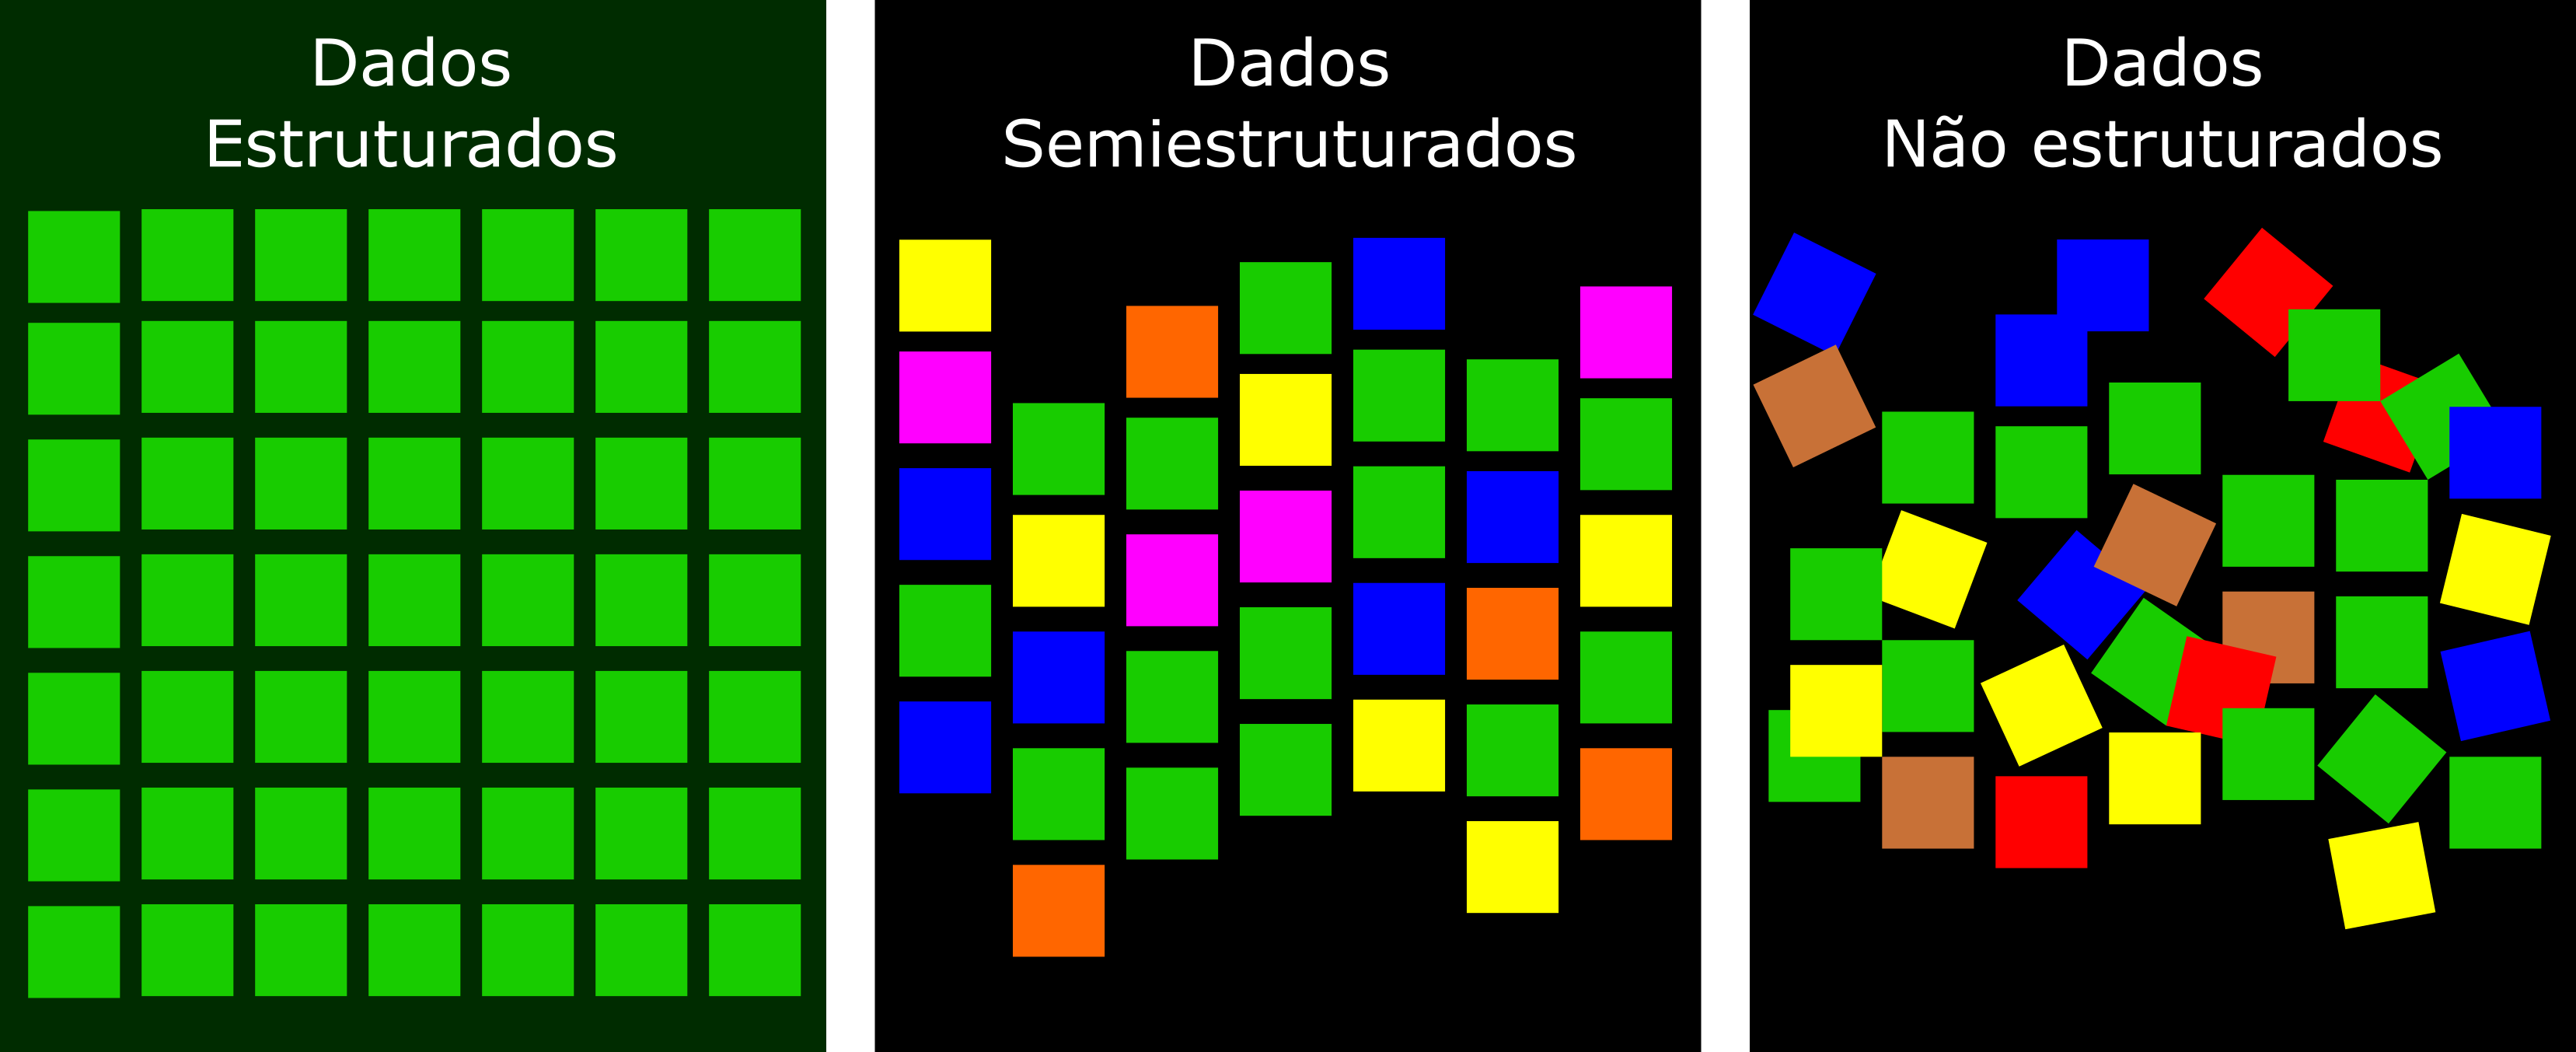
\includegraphics[width=0.9\textwidth]{figuras/dados.png}
					\label{fig:identificador_da_figura}
					\fonte{Autor}
				} 		
			\end{figure}

		\obs{Isso é uma observação para conversar com o orientador ou para recordação}

		Utilize esse comando para tachar um texto, exemplo: \tachado{comprar}adquirir.
		\subsection{Subseção}
		\label{subsec:subseçao}
			Bla bla bla


% Base Teórica
\chapter{Título do Capítulo}
\label{ch:identificador}
	\begin{resumocapitulo}
		Aqui vai um pequeno resumo do capítulo.
	\end{resumocapitulo}

	\section{Visão Geral}
		Descrever uma visão do capítulo. É um resumo mais elaborado que visa posicionar o leitor sobre o que será abordado adiante.

	\section{Conteúdo 1}
	\label{sec:identificao}
        Bla bla

		% Lista numerada
		\begin{enumerate}
			\item Bla
			\item Bla
		\end{enumerate}

		% Lacuna de pesquisa - um bloco para cada lacuna
		\begin{lacuna}
		\label{lacuna:lacuna1}
			Descrever aqui a lacuna de pesquisa. Se tiver mais que uma, criar outro bloco.
		\end{lacuna}
	
		% Pergunta de pesquisa - um bloco para cada pergunta
		\begin{pergunta}
		\label{pergunta:pergunta_1}
			Aqui vai a pergunta de pesquisa 1.
		\end{pergunta}

		\begin{pergunta}
		\label{pergunta:pergunta_2}
			Aqui vai a pergunta de pesquisa 2.
		\end{pergunta}

% Conclusão
\chapter{Conclusões}
\label{ch:conclusao}
	Descrever as conclusões do trabalho... bla bla bla.

% Trabalhos Futuros
\chapter{Trabalhos Futuros}
\label{ch:trabalhos_futuros}
	Descrever os trabalhos futuros.

	\begin{enumerate}
		\item Texto
		\item Texto
		\item Texto
	\end{enumerate}


% ##################### Fim dos Capítulos ############################

% Bibliografia (Obrigatório)
\bibliography{refs}

% ##################### Apêndices ############################
\renewcommand{\appendixtitle}{Apêndices}
\begin{appendixenv}
    \section{: Título}
    \subsection*{Descrição}
        \begin{enumerate}
            \item Conteúdo
        \end{enumerate}        
        

\end{appendixenv}

% ##################### Anexos ############################
\renewcommand{\appendixtitle}{Anexos}
\begin{appendixenv}
    \section{: Título}
    \subsection*{Publicação}
        \begin{enumerate}
            \item DE SOUZA, E. M.; STOROPOLI, J. E. ; ALVES, W. A. L.~\textbf{FERRAMENTA DE EXTRAÇÃO DE DADOS PARA A WEB OF SCIENCE}. \textbf{In}: SETII - Seminário em Tecnologia da Informação Inteligente, 2019, São Paulo. Universidade Nove de Julho.
        \end{enumerate}
\end{appendixenv}

\end{document}